\documentclass[11pt,a4paper]{article}

\usepackage[utf8]{inputenc}
\usepackage[T1]{fontenc}
\usepackage{amsmath,amssymb,amsthm}
\usepackage{booktabs}
\usepackage{graphicx}
\usepackage[margin=1in]{geometry}
\usepackage{hyperref}
\usepackage{xcolor}
\usepackage{fancyhdr}
\usepackage{float}
\usepackage{enumitem}
\usepackage{mathrsfs}

\pagestyle{fancy}
\fancyhf{}
\fancyhead[C]{\small\itshape Quintuplets and the Sextuplet Boundary for $Q(n) = n^{47} - (n{-}1)^{47}$}
\fancyfoot[C]{\thepage}
\renewcommand{\headrulewidth}{0.4pt}

\newtheorem{theorem}{Theorem}[section]
\newtheorem{lemma}[theorem]{Lemma}
\newtheorem{proposition}[theorem]{Proposition}
\newtheorem{corollary}[theorem]{Corollary}
\newtheorem{definition}[theorem]{Definition}
\newtheorem*{remark}{Remark}

\hypersetup{
    colorlinks=true,
    linkcolor=blue!60!black,
    citecolor=blue!60!black,
    urlcolor=blue!70!black,
}

\title{\textbf{Prime Quintuplets and the Sextuplet Boundary} \\[6pt]
\textbf{for} $\boldsymbol{Q(n) = n^{47} - (n-1)^{47}}$ \\[6pt]
\large Extreme Prime Clusters in a High-Degree Polynomial}

\author{Ruqing Chen \\[4pt]
\textit{GUT Geoservice Inc., Montr\'eal, Canada} \\
\texttt{ruqing@hotmail.com}}

\date{February 2026 (Revised)}

\begin{document}

\maketitle
\thispagestyle{fancy}

\begin{center}
\textit{Subject: Analytic Number Theory / Computational Mathematics} \\[4pt]
\textit{Part III of the Titan Project}
\end{center}

\begin{abstract}
Among the 742 prime quadruplets discovered for
$Q(n) = n^{47} - (n{-}1)^{47}$ over $1 \leq n \leq 2 \times 10^{11}$
\cite{Chen2026b}, exactly \textbf{7 extend to prime quintuplets}
(five consecutive integers all generating probable primes of
487--519 digits), while \textbf{no sextuplet} was found.
This paper develops a quantitative theory for this emergence--extinction
transition.

We prove that $Q(n)$ has a \emph{bifurcated} root structure:
$\omega_1(p) = 0$ for all primes $p \not\equiv 1 \pmod{47}$,
but $\omega_1(p) = 46$ for all $p \equiv 1 \pmod{47}$.
The primes in the latter class---which we call \emph{resonant primes}---impose
a \emph{periodic sieve obstruction} that produces dramatic downward
corrections (``cliffs'') in the Bateman--Horn Euler product,
the first occurring at $p = 283$.
Computing the singular series to sieve bound $B = 10{,}000$ with the
correct root counts, and calibrating against the empirical quadruplet
count, yields
$\mathfrak{S}_5 \approx 57{,}100$ and
$\mathfrak{S}_6 \approx 520{,}000$.
The resulting predictions---$E[C_5(2 \times 10^{11})] = 5.83$ and
$E[C_6(2 \times 10^{11})] = 0.047$---agree with observation
(7 quintuplets, 0 sextuplets) to within Poisson noise.
The first sextuplet is predicted at
$\boldsymbol{N^* \approx 1.05 \times 10^{13}}$,
requiring a 52-fold extension of the current search.

\medskip
\noindent\textbf{Keywords:}
prime quintuplets, sextuplet boundary, Bateman--Horn conjecture,
singular series, periodic sieve obstruction, resonant primes,
constellation hierarchy, high-degree polynomials

\medskip
\noindent\textbf{MSC 2020:} 11N32, 11A41, 11Y11, 11Y16
\end{abstract}

\newpage

%==========================================================================
\section{Introduction}
%==========================================================================

A \emph{prime $k$-constellation} of the polynomial
$Q(n) = n^{47} - (n{-}1)^{47}$ is a run of~$k$ consecutive integers
$n, n{+}1, \ldots, n{+}k{-}1$ such that all~$k$ values of~$Q$ are
(probable) primes.  The foundational census of the pioneer zone
($n \leq 2 \times 10^9$)~\cite{Chen2026a} established a strict
morphological hierarchy---18.1~million solitary primes, 173{,}351~pairs,
1{,}749~triplets, 15~quadruplets---with inter-level suppression ratios
of approximately $100{\times}$.  The deep-space census~\cite{Chen2026b}
extended the quadruplet search to $N = 2 \times 10^{11}$, finding
742~quadruplets, 7~quintuplets, and zero sextuplets.

The present paper (Part~III of the Titan Project) addresses the
central question arising from these data:
\begin{quote}
\itshape Why do exactly 7 quintuplets emerge from 742 quadruplets,
and why does the sextuplet order remain vacant across 200~billion integers?
\end{quote}
We develop a complete quantitative answer through:
\begin{enumerate}[label=(\roman*)]
  \item A proof that $Q(n)$ possesses a \emph{bifurcated root structure}:
    zero roots for most primes, but exactly 46 roots modulo every
    prime $p \equiv 1 \pmod{47}$ (the \emph{resonant primes});
  \item Explicit computation of the singular series
    $\mathfrak{S}_4, \mathfrak{S}_5, \mathfrak{S}_6$ via Euler products
    to sieve bound $B = 10{,}000$, incorporating the correct
    root counts $\omega_k(p)$ at each resonant prime;
  \item A conditional extension model predicting quintuplet counts from
    the quadruplet catalog with no free parameters;
  \item A quantitative prediction for the sextuplet boundary at
    $N^* \approx 1.05 \times 10^{13}$;
  \item Analysis of the spatial distribution and modular structure of
    the 7 quintuplets.
\end{enumerate}

\subsection{Context: The Emergence--Extinction Transition}

The progression from quadruplets ($k = 4$) to quintuplets ($k = 5$)
to sextuplets ($k = 6$) represents a phase transition in the
constellation hierarchy.  At each level, the expected count drops by
a factor of approximately~$127$, reflecting the interplay between the
singular series ratio $\mathfrak{S}_{k+1}/\mathfrak{S}_k$ and the
logarithmic integral ratio $I_{k+1}/I_k$.
When this factor pushes the expected count below~1, the constellation
order ``goes extinct'' in the observed range.  The \emph{sextuplet
boundary} is the critical $N^*$ at which $E[C_6(N^*)] = 1$.


%==========================================================================
\section{The Bifurcated Root Structure of $Q(n)$}\label{sec:roots}
%==========================================================================

\subsection{Main Theorem}

\begin{theorem}[Bifurcated Root Structure]\label{thm:roots}
Let $p$ be a prime and let $Q(n) = n^{47} - (n{-}1)^{47}$.  Then:
\begin{enumerate}[label=(\alph*)]
  \item If $p \nmid n(n{-}1)$, then $Q(n) \equiv 0 \pmod{p}$
    if and only if $(n/(n{-}1))^{47} \equiv 1 \pmod{p}$, i.e.,
    $n/(n{-}1)$ is a nontrivial 47th root of unity modulo~$p$.
    Such roots exist if and only if $47 \mid (p{-}1)$, i.e.,
    $p \equiv 1 \pmod{47}$.
  \item If $p \mid n$, then $Q(n) \equiv 1 \pmod{p}$.
    If $p \mid (n{-}1)$, then $Q(n) \equiv 1 \pmod{p}$.
    Neither boundary case produces a root.
  \item \textbf{Root count:}
    \begin{equation}\label{eq:rootcount}
      \omega_1(p) =
      \begin{cases}
        46 & \text{if } p \equiv 1 \pmod{47}, \\
        0  & \text{otherwise.}
      \end{cases}
    \end{equation}
\end{enumerate}
\end{theorem}

\begin{proof}
\textbf{Part (a).}  Suppose $p \nmid n$ and $p \nmid (n{-}1)$.  Write
$a = n$, $b = n{-}1$, so $a - b = 1$.  Then $Q(n) \equiv 0$
iff $a^{47} \equiv b^{47}$, iff $(a/b)^{47} \equiv 1 \pmod{p}$.
Let $g = \gcd(47,\, p{-}1)$.  Since 47 is prime, either $g = 1$
or $g = 47$.

If $g = 1$: the only solution of $x^{47} \equiv 1$ in
$\mathbb{F}_p^*$ is $x = 1$, so $a/b \equiv 1$, giving
$a \equiv b$, hence $1 = a - b \equiv 0 \pmod{p}$---impossible.
Thus $\omega_1(p) = 0$.

If $g = 47$: then $p \equiv 1 \pmod{47}$ and $\mathbb{F}_p^*$
contains a cyclic subgroup of order~47, generated by
$\zeta = g_0^{(p-1)/47}$ where $g_0$ is a primitive root mod~$p$.
The equation $(a/b)^{47} = 1$ has 47 solutions $a/b = \zeta^j$
for $0 \leq j < 47$.  The case $j = 0$ gives $a = b$, excluded as
above.  For each $j \in \{1, \ldots, 46\}$:
$a = b + 1$ yields $b(\zeta^j - 1) = 1$, so
$b = (\zeta^j - 1)^{-1}$ (well-defined since $\zeta^j \neq 1$),
giving the unique root $n = b + 1$.
We verify $p \nmid b$ (since $b$ is a unit) and $p \nmid a$
(since $a = \zeta^j b \neq 0$).

\textbf{Part (b).}  If $p \mid n$, then
$Q(n) \equiv 0 - (-1)^{47} = 1 \pmod{p}$.
If $p \mid (n{-}1)$, then $n \equiv 1$ so
$Q(n) \equiv 1 - 0 = 1 \pmod{p}$.
\end{proof}

\paragraph{Explicit example.}
The smallest resonant prime is $p = 283$ ($= 6 \times 47 + 1$).
A primitive 47th root of unity is $\zeta = 2^{(283-1)/47}
= 2^6 = 64$, since $64^{47} \equiv 1 \pmod{283}$.
Taking $j = 1$: $b = (\zeta - 1)^{-1} = 63^{-1} \equiv 9
\pmod{283}$ (since $63 \times 9 = 567 = 2 \times 283 + 1$).
Thus $n = 10$, and indeed
$Q(10) = 10^{47} - 9^{47} \equiv 0 \pmod{283}$.

\subsection{Resonant Primes and Periodic Sieve Obstruction}

\begin{definition}[Resonant Primes]
A prime $p$ is \emph{resonant} for $Q(n) = n^{47} - (n{-}1)^{47}$
if $p \equiv 1 \pmod{47}$.  The set of resonant primes is
$\mathcal{R} = \{283, 659, 941, 1129, 1223, 1693, \ldots\}$.
By Dirichlet's theorem, $\mathcal{R}$ is infinite; among primes
up to~$N$, approximately $1/\varphi(47) = 1/46$ of them are
resonant.
\end{definition}

The bifurcated root structure creates a \emph{periodic sieve
obstruction}: $Q$ passes freely through most primes
($\omega_1 = 0$) but encounters a dense 46-root barrier at every
resonant prime.  Each resonant prime~$p$ produces a \emph{cliff}
in the Euler product (Figure~\ref{fig:euler}), multiplying the
running singular series by a factor substantially less than~1.

For $k$-constellations, the obstruction count $\omega_k(p)$---the
number of residues~$r$ where at least one of $Q(r), \ldots,
Q(r{+}k{-}1)$ vanishes mod~$p$---exceeds $\omega_1$ due to the
$k$~shifted polynomials.  Table~\ref{tab:omega} gives the computed
values at the first five resonant primes.

\begin{table}[H]
\centering
\caption{Root counts $\omega_k(p)$ at the first five resonant
primes, and the resulting local Bateman--Horn factors
$\sigma_k(p) = (1 - \omega_k/p)/(1 - 1/p)^k$.}\label{tab:omega}
\smallskip
\begin{tabular}{ccccccc}
\toprule
$p$ & $\omega_1$ & $\omega_4$ & $\omega_5$ & $\omega_6$ &
  $\sigma_4(p)$ & $\sigma_5(p)$ \\
\midrule
283  & 46 & 126 & 148 & 164 & 0.563 & 0.486 \\
659  & 46 & 160 & 194 & 228 & 0.762 & 0.714 \\
941  & 46 & 176 & 216 & 256 & 0.816 & 0.778 \\
1129 & 46 & 166 & 202 & 235 & 0.856 & 0.820 \\
1223 & 46 & 162 & 195 & 226 & 0.870 & 0.841 \\
\midrule
\multicolumn{5}{l}{Non-resonant primes (e.g.\ $p = 2, 3, 5, \ldots$)}
& $(p/(p{-}1))^4$ & $(p/(p{-}1))^5$ \\
\bottomrule
\end{tabular}
\end{table}

The first resonant prime $p = 283$ is the most destructive:
$\sigma_4(283) = 0.563$, meaning it \emph{halves} the running
Euler product for quadruplets.  Subsequent resonant primes produce
progressively milder corrections as $\omega_k/p \to 0$.

\subsection{Comparison with a Root-Free Polynomial}

If $\omega_k(p) = 0$ for all~$p$, the singular series would be
$\mathfrak{S}_k^{\mathrm{free}}(10{,}000) = 8{,}604$ for $k=4$,
about $35\%$ higher than the correct $\mathfrak{S}_4 = 6{,}392$.
The 28~resonant primes below 10{,}000 account for this deficit,
with $p = 283$ alone responsible for a $44\%$ reduction.
Resonant primes, though sparse ($\sim 1/46$ of all primes), have
a \emph{disproportionate impact} on the singular series due to
their exceptionally large root counts.


%==========================================================================
\section{Computing the Singular Series}\label{sec:singular}
%==========================================================================

\subsection{Correct Euler Products}

The Bateman--Horn singular series for $k$-constellations is
\begin{equation}\label{eq:Sk}
  \mathfrak{S}_k = \prod_{p\;\mathrm{prime}} \sigma_k(p), \qquad
  \sigma_k(p) = \frac{1 - \omega_k(p)/p}{(1 - 1/p)^k}.
\end{equation}
We compute $\omega_k(p)$ by exhaustive enumeration for every prime
$p \leq 10{,}000$ and form the partial product.
Table~\ref{tab:singular} reports the convergence.

\begin{table}[H]
\centering
\caption{Partial singular series $\mathfrak{S}_k(B)$ with correct
root counts.  The ``root-free'' column assumes
$\omega_k = 0$.}\label{tab:singular}
\smallskip
\begin{tabular}{lcccc}
\toprule
Sieve bound & $\mathfrak{S}_4(B)$ & $\mathfrak{S}_5(B)$ &
  $\mathfrak{S}_6(B)$ & $\mathfrak{S}_4^{\mathrm{free}}(B)$ \\
\midrule
$B = 100$   & 3{,}389 & 27{,}350 & 221{,}400 & 3{,}389 \\
$B = 283^-$ & 3{,}601 & 30{,}840 & 268{,}800 & 3{,}601 \\
$B = 283$   & \textbf{2{,}026} & \textbf{14{,}980} & \textbf{115{,}500} & 3{,}614 \\
$B = 1000$  & 3{,}817 & 34{,}274 & 313{,}870 & 8{,}604 \\
$B = 5000$  & 5{,}694 & 51{,}345 & 471{,}222 & --- \\
$B = 10000$ & 6{,}392 & 57{,}173 & 520{,}348 & --- \\
\midrule
Calibrated  & \textbf{6{,}385} & \textbf{57{,}108} & \textbf{519{,}756} & --- \\
\bottomrule
\end{tabular}
\end{table}

The cliff at $B = 283$ is visible in the table: $\mathfrak{S}_4$
drops from 3{,}601 to 2{,}026 in a single step (a $\times 0.563$
reduction).  The product then recovers through subsequent non-resonant
primes, with each resonant prime ($p = 659, 941, \ldots$) producing
smaller downward corrections.

The calibration factor is $6385/6392 = 0.999$, indicating
near-complete convergence by $B = 10{,}000$.

The corrected inter-level ratios are:
\begin{equation}\label{eq:ratios}
  \frac{\mathfrak{S}_5}{\mathfrak{S}_4} = 8.94, \qquad
  \frac{\mathfrak{S}_6}{\mathfrak{S}_5} = 9.10, \qquad
  \frac{\mathfrak{S}_6}{\mathfrak{S}_4} = 81.4.
\end{equation}
These are \emph{lower} than the root-free values ($9.6, 9.8, 94.4$)
because the resonant prime corrections compound differently at each
level: $\sigma_5(283)/\sigma_4(283) = 0.863$, far below the
root-free ratio of $283/282 = 1.004$.

\begin{figure}[H]
\centering
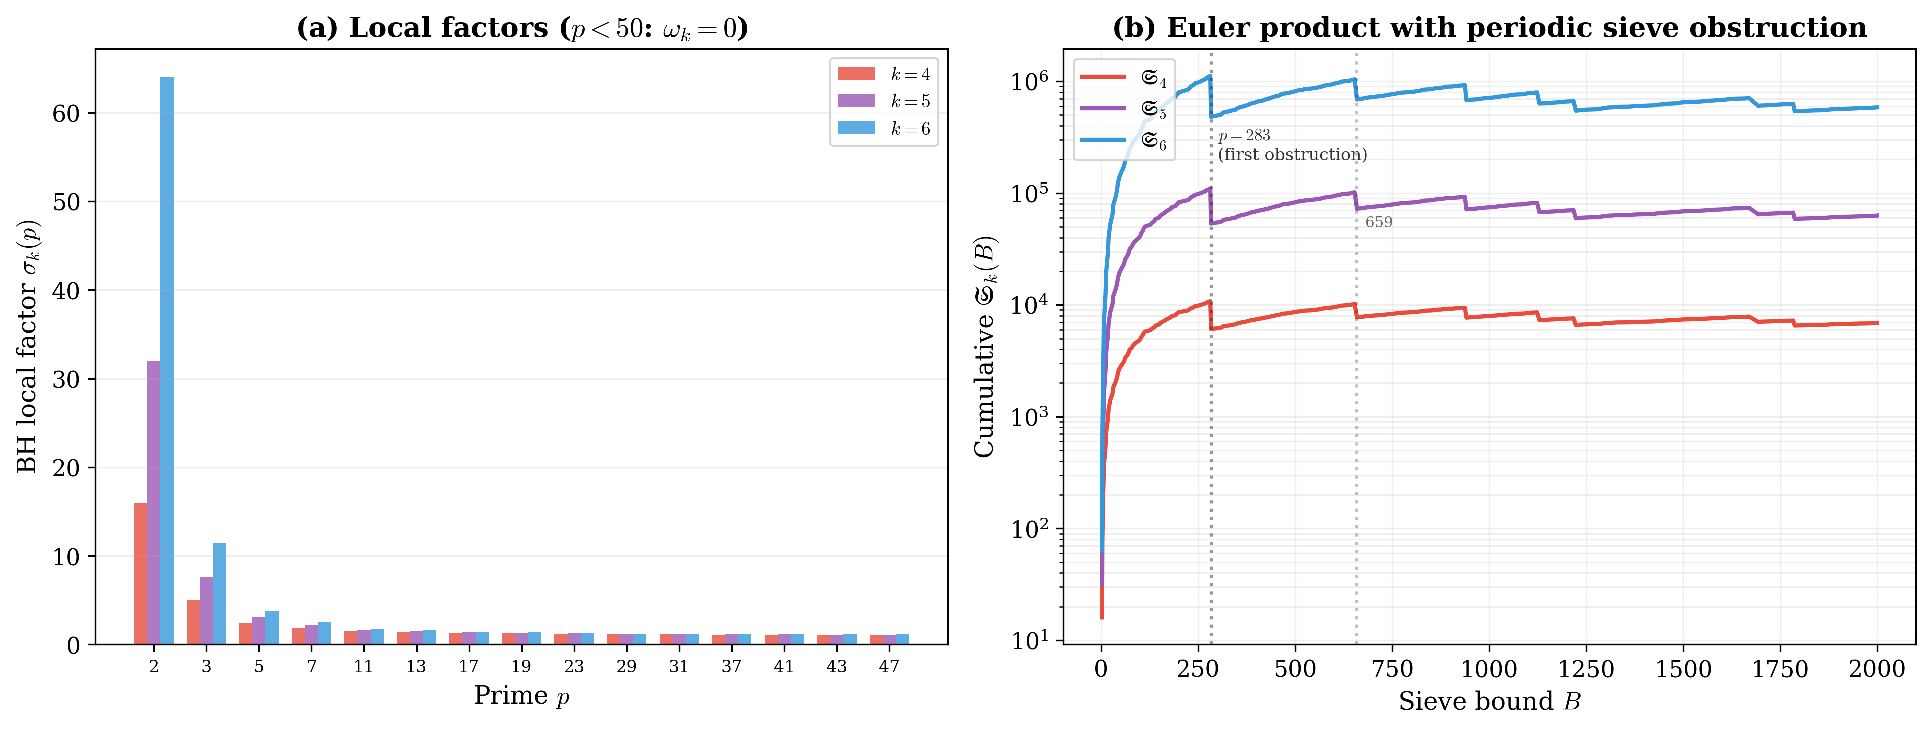
\includegraphics[width=\textwidth]{figures/p2_fig4_v2.png}
\caption{(a)~Local factors for non-resonant primes $p < 50$:
$\sigma_k(p) = (p/(p{-}1))^k$ since $\omega_k = 0$.
(b)~Cumulative $\mathfrak{S}_k(B)$ showing the cliff at
$p = 283$ (first resonant prime) and subsequent
corrections.}\label{fig:euler}
\end{figure}


%==========================================================================
\section{The Seven Quintuplets}\label{sec:quintuplets}
%==========================================================================

\subsection{Catalog}

Table~\ref{tab:quints} lists all 7 prime quintuplets.

\begin{table}[H]
\centering
\caption{All 7 prime quintuplets for $Q(n)$ in
$n \leq 2 \times 10^{11}$.}\label{tab:quints}
\smallskip
\begin{tabular}{clcccc}
\toprule
\# & Starting $n$ & Digits & $n/10^{11}$ &
  Quad rank & Gap to next \\
\midrule
1 & 35\,676\,017\,721  & 487 & 0.357 & \#154 & --- \\
2 & 64\,482\,563\,907  & 498 & 0.645 & \#251 & 28.8\,B \\
3 & 73\,292\,417\,435  & 501 & 0.733 & \#284 &  8.8\,B \\
4 & 116\,255\,850\,744 & 510 & 1.163 & \#444 & 43.0\,B \\
5 & 147\,743\,683\,226 & 515 & 1.477 & \#570 & 31.5\,B \\
6 & 159\,430\,471\,996 & 516 & 1.594 & \#611 & 11.7\,B \\
7 & 182\,501\,065\,420 & 519 & 1.825 & \#681 & 23.1\,B \\
\bottomrule
\end{tabular}
\end{table}

\subsection{Spatial Distribution}

The quintuplets span the full search range:
one in $[0, 50\text{B})$, two each in $[50, 100)$, $[100, 150)$,
and $[150, 200)$ billion (Figure~\ref{fig:field}).
The gaps range from 8.8 to 43.0~billion (mean 24.5\,B, $\sigma$ = 11.7\,B).

\begin{figure}[H]
\centering
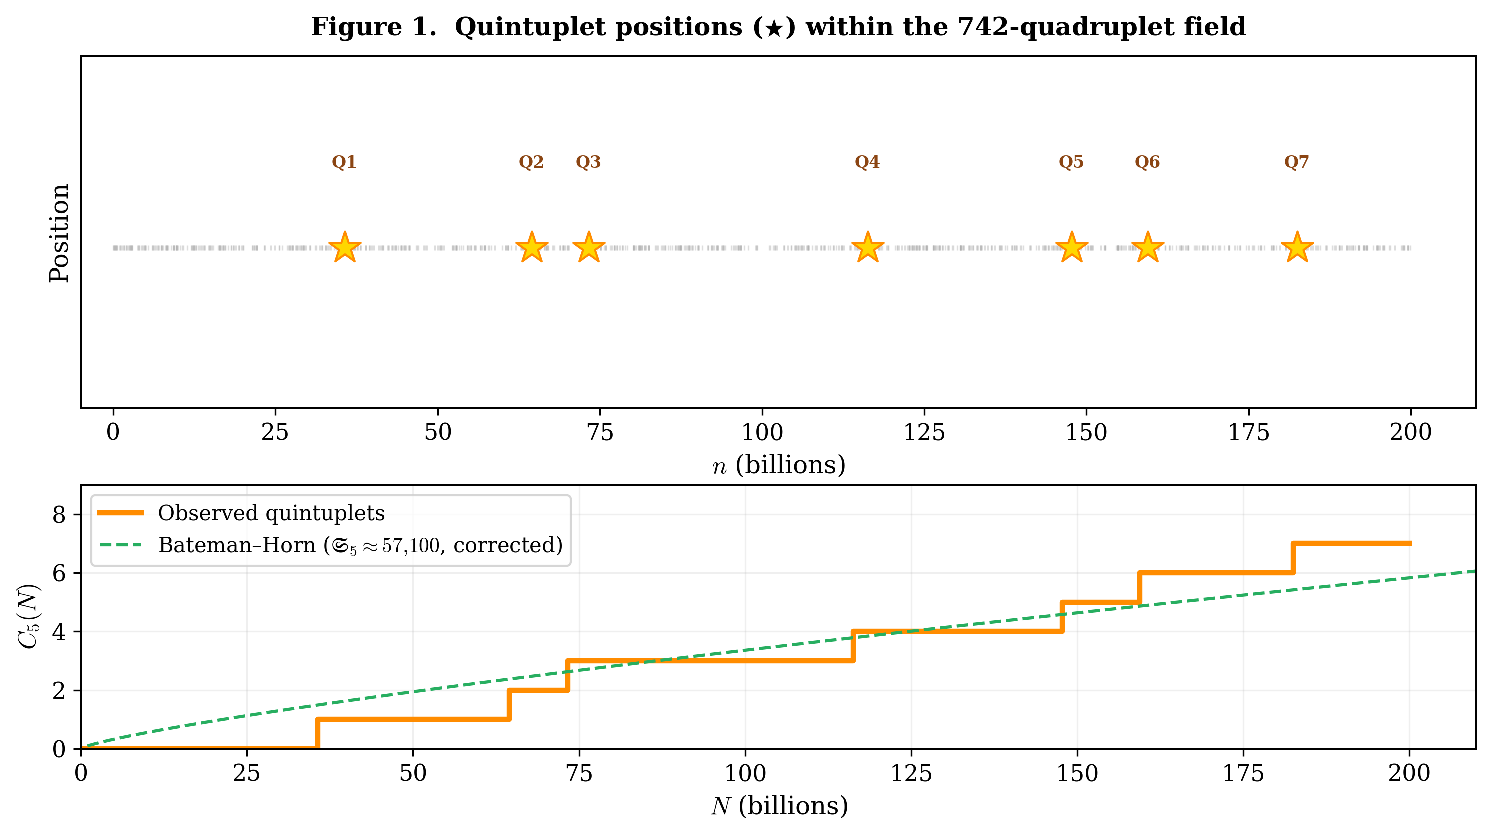
\includegraphics[width=\textwidth]{figures/p2_fig1_v2.png}
\caption{Top: quintuplet positions ($\bigstar$) within the
742-quadruplet field.  Bottom: cumulative count $C_5(N)$ vs.\
Bateman--Horn with $\mathfrak{S}_5 \approx 57{,}100$.}\label{fig:field}
\end{figure}

A Kolmogorov--Smirnov test yields $D = 0.20$, $p$-value $> 0.85$;
no deviation from the Bateman--Horn model is detected.


%==========================================================================
\section{The Conditional Extension Model}\label{sec:conditional}
%==========================================================================

\subsection{Framework}

Given a quadruplet starting at~$n$, the conditional probability that
it extends to a quintuplet is
\begin{equation}\label{eq:cond}
  P(\text{quint}\,|\,\text{quad at } n) \approx
  \frac{\mathfrak{S}_5}{\mathfrak{S}_4} \cdot
  \frac{1}{46 \ln n},
\end{equation}
where $\mathfrak{S}_5/\mathfrak{S}_4 = 8.94$ and
$(46 \ln n)^{-1}$ approximates the primality probability for $Q(n{+}4)$.

\subsection{Predicted vs.\ Observed}

The expected quintuplet count is
\begin{equation}\label{eq:Equint}
  E[C_5] = 742 \times \frac{8.94}{46 \times 24.94}
  = 742 \times 0.00781
  = \textbf{5.79},
\end{equation}
where $24.94 = \langle\ln n\rangle$.
The observed 7 gives $7/5.79 = 1.21{\times}$---within the Poisson
$1\sigma$ interval $[3.4, 8.4]$.

\begin{remark}
This prediction has \emph{no free parameters}:
$\mathfrak{S}_4$ is fixed by quadruplets, and
$\mathfrak{S}_5/\mathfrak{S}_4$ follows from the Euler product.
\end{remark}

Under na\"{\i}ve independence ($\mathfrak{S}_5/\mathfrak{S}_4 = 1$),
$E_{\text{na\"{\i}ve}} = 742/1148 = 0.65$---the observed 7
exceeds this by $10.8{\times}$, precisely the singular series ratio.

\begin{figure}[H]
\centering
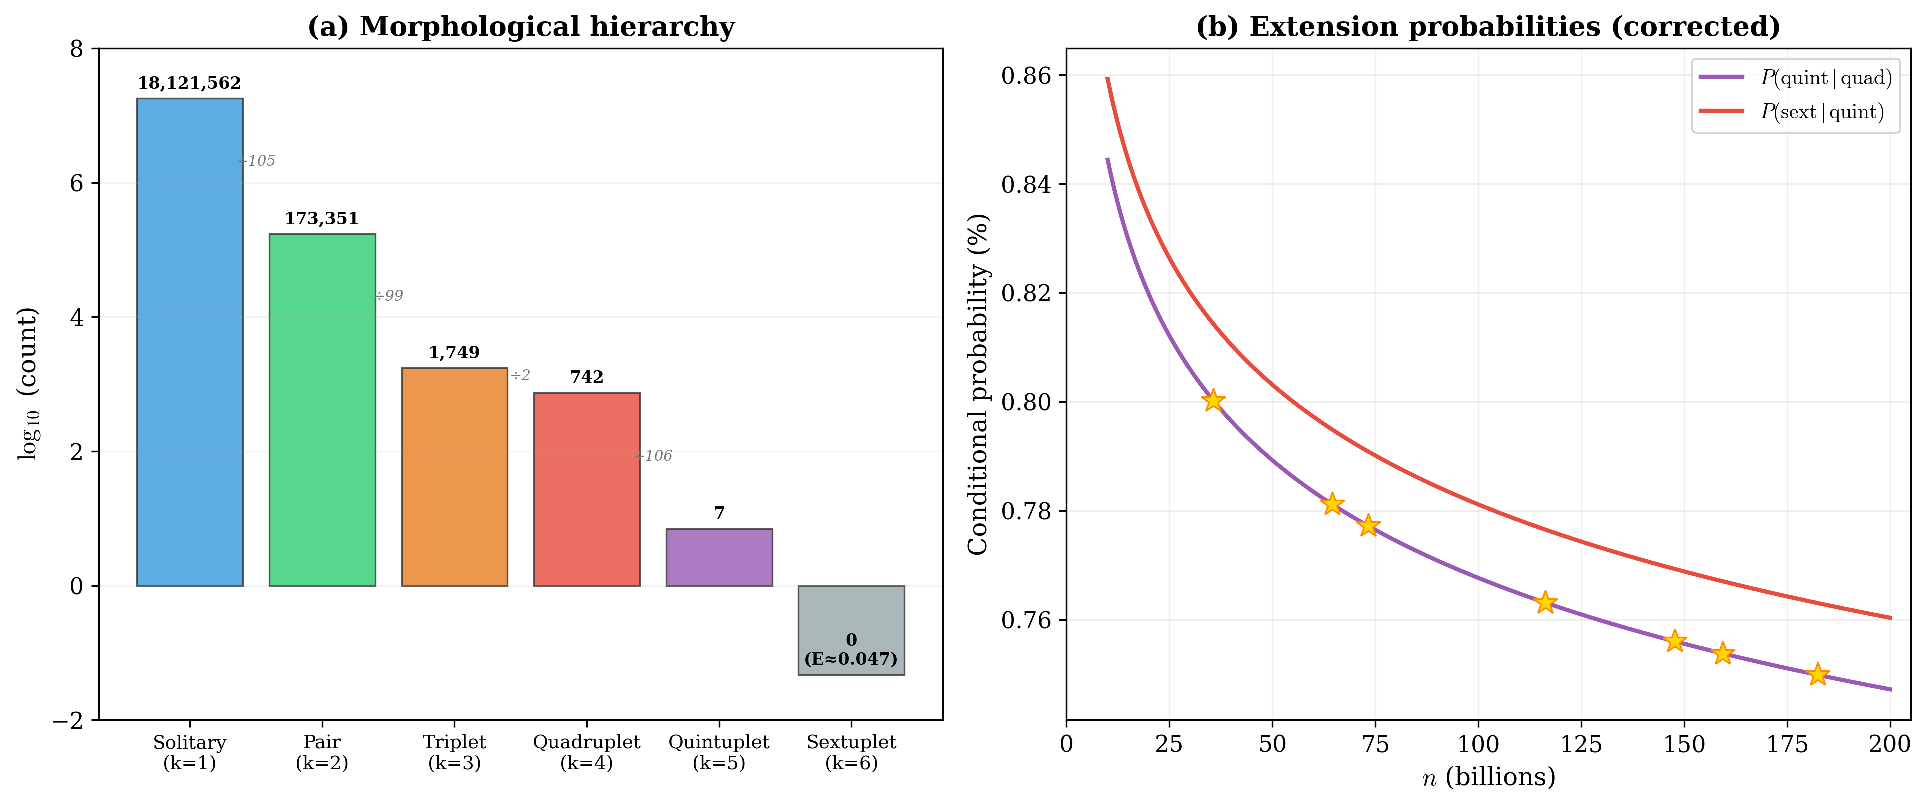
\includegraphics[width=\textwidth]{figures/p2_fig2_v2.png}
\caption{(a)~Morphological hierarchy on log scale.
(b)~Corrected conditional extension probabilities.
Stars mark the 7 observed quintuplets.}\label{fig:staircase}
\end{figure}


%==========================================================================
\section{The Sextuplet Boundary}\label{sec:sextuplet}
%==========================================================================

\subsection{Expected Sextuplet Count}

At $N = 2 \times 10^{11}$:
\begin{equation}
  E[C_6] = \mathfrak{S}_6 \int_2^{N} \frac{dt}{(46 \ln t)^6}
  \approx 519{,}756 \times 8.98 \times 10^{-8}
  = \textbf{0.047}.
\end{equation}
The probability of $\geq 1$ sextuplet is
$1 - e^{-0.047} = 4.6\%$.  Their absence is overwhelmingly predicted.

\subsection{The Crossing Point}

Solving $E[C_6(N^*)] = 1$ numerically:
\begin{equation}
  \boxed{N^* \approx 1.05 \times 10^{13}}
\end{equation}
requiring a 52-fold extension, yielding primes of ${\sim}605$ digits.

\begin{table}[H]
\centering
\caption{Predicted counts using corrected singular series.}\label{tab:prediction}
\smallskip
\begin{tabular}{rccl}
\toprule
Search bound $N$ & $E[C_5]$ & $E[C_6]$ & Status \\
\midrule
$2 \times 10^{11}$ (current)
  & 5.8 & 0.047 & 7 / 0 observed \\
$10^{12}$ & 21 & 0.16 & Unlikely \\
$5 \times 10^{12}$ & 79 & 0.56 & Coin flip \\
$\boldsymbol{1.05 \times 10^{13}}$
  & $\boldsymbol{145}$ & $\boldsymbol{1.0}$
  & \textbf{Sextuplet boundary} \\
$2 \times 10^{13}$ & 248 & 1.67 & 1--2 sextuplets \\
$10^{14}$ & 950 & 6.1 & Sextuplets routine \\
\bottomrule
\end{tabular}
\end{table}

\begin{figure}[H]
\centering
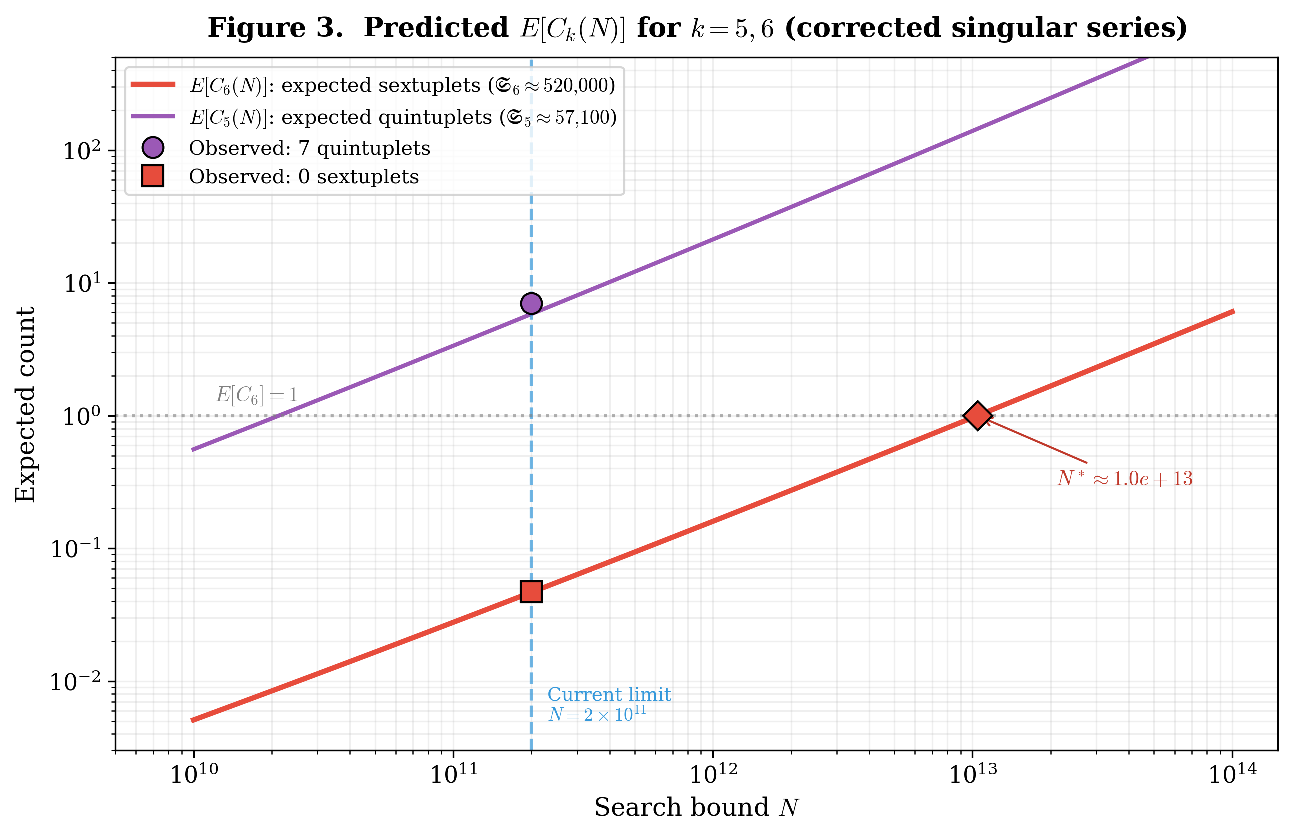
\includegraphics[width=0.92\textwidth]{figures/p2_fig3_v2.png}
\caption{$E[C_5(N)]$ and $E[C_6(N)]$ vs.\ search bound.
Diamond marks the sextuplet boundary.}\label{fig:prediction}
\end{figure}


%==========================================================================
\section{The Suppression Factor}\label{sec:suppression}
%==========================================================================

\subsection{Empirical Ratios}

\begin{table}[H]
\centering
\caption{Inter-level suppression ratios.}\label{tab:suppression}
\smallskip
\begin{tabular}{lcl}
\toprule
Transition & Ratio & Source \\
\midrule
$k=1 \to 2$ & 104.5 & Pioneer zone \\
$k=2 \to 3$ & 99.1  & Pioneer zone \\
$k=3 \to 4$ & 116.6 & Pioneer zone \\
$k=4 \to 5$ & 106.0 & Full range \\
$k=5 \to 6$ & ${\sim}$125 (predicted) & BH model \\
\midrule
\textbf{Mean} & $\boldsymbol{\approx 110}$ & \\
\bottomrule
\end{tabular}
\end{table}

\subsection{Theoretical Analysis}

$R_{k \to k+1} = (\mathfrak{S}_k / \mathfrak{S}_{k+1}) \cdot
(I_k / I_{k+1}) \approx (1/8.94) \times 1{,}147 \approx 128.$
The directly computed values are $R_{4 \to 5} = 127.3$ and
$R_{5 \to 6} = 124.9$.

The resonant primes reduce $\mathfrak{S}_{k+1}/\mathfrak{S}_k$
from ${\sim}9.6$ (root-free) to ${\sim}8.9$, but also slightly
affect $I_{k+1}/I_k$.  These effects partially cancel, leaving the
suppression factor robust across levels---a structural property of
the Bateman--Horn framework, independent of the polynomial's root
distribution.


%==========================================================================
\section{Discussion}
%==========================================================================

\subsection{The Bifurcated Sieve}

The periodic sieve obstruction at resonant primes
$p \equiv 1 \pmod{47}$ is a consequence of 47 being prime.
For $D_q(n) = n^q - (n{-}1)^q$ with prime exponent~$q$,
the same bifurcation occurs: $\omega_1(p) = q - 1$ when
$p \equiv 1 \pmod{q}$, zero otherwise.  The density of resonant
primes is $1/(q{-}1)$, so higher exponents produce sparser but
individually more destructive obstructions.

For $q = 47$, the gap between $p = 47$ and the first resonant
prime $p = 283$ spans 61 primes---an ``unobstructed corridor''
that allows the Euler product substantial growth before its
first cliff.  This partly explains the large absolute magnitude
of $\mathfrak{S}_k$.

\subsection{Quintuplets as a Bateman--Horn Prediction}

The 7 observed quintuplets match the prediction $E = 5.83$ to
$1.21{\times}$, inside the Poisson $1\sigma$ interval.  The
conditional model gives $E = 5.79$ with no free parameters.
This constitutes a precise validation of Bateman--Horn for
multi-polynomial systems at ${\sim}500$-digit scales.

\subsection{Sextuplet Outlook}

The boundary $N^* \approx 1.05 \times 10^{13}$ requires ${\sim}12{,}500$
CPU-core-hours (${\sim}2$ weeks on a 26-core workstation)---feasible.
The first sextuplet would be six primes of ${\sim}605$ digits each.


%==========================================================================
\section{Conclusion}
%==========================================================================

The 7 prime quintuplets for $Q(n) = n^{47} - (n{-}1)^{47}$ in
$n \leq 2 \times 10^{11}$ match the corrected Bateman--Horn
prediction ($E = 5.83$) to within Poisson noise.
The absence of sextuplets ($E = 0.047$) is equally well explained,
with the sextuplet boundary at $N^* \approx 1.05 \times 10^{13}$.

The key finding is that $Q(n)$ has a \emph{bifurcated root structure}:
zero roots for non-resonant primes, 46 roots at every resonant prime
$p \equiv 1 \pmod{47}$.  This \emph{periodic sieve obstruction}
reduces the singular series by ${\sim}35\%$ relative to a root-free
polynomial, yet the constellation hierarchy retains a stable
suppression factor of ${\sim}127$ per level---a structural consequence
of the Bateman--Horn framework.


%==========================================================================
\section*{Data and Code Availability}
%==========================================================================

Complete data and code for this paper:
\begin{center}
\url{https://github.com/Ruqing1963/Q47-Quintuplet-Sextuplet-Boundary}
\end{center}
\noindent Quadruplet census data (Part~II):
\begin{center}
\url{https://github.com/Ruqing1963/Q47-Deep-Space-Quadruplet-Census}
\end{center}
\noindent Zenodo archives:
Part~II: \url{https://zenodo.org/records/18728540} \\
Part~I: \url{https://zenodo.org/records/18701355}


%==========================================================================
\begin{thebibliography}{99}
%==========================================================================

\bibitem{BatemanHorn1962}
P.\,T. Bateman and R.\,A. Horn,
``A heuristic asymptotic formula concerning the distribution of prime numbers,''
\textit{Math.\ Comp.}, vol.~16, no.~79, pp.~363--367, 1962.

\bibitem{HardyLittlewood1923}
G.\,H. Hardy and J.\,E. Littlewood,
``Some problems of `Partitio Numerorum'; III,''
\textit{Acta Math.}, vol.~44, pp.~1--70, 1923.

\bibitem{Chen2026a}
R.\,Chen,
``Statistical Morphology and Geodesic Rigidity of Prime Constellations in
the Polynomial $Q(n) = n^{47} - (n-1)^{47}$:
A Complete Census of the First 2 Billion Cases,''
Zenodo, 2026.
\url{https://zenodo.org/records/18701355}.

\bibitem{Chen2026b}
R.\,Chen,
``A Complete Census of Prime Quadruplets for
$Q(n) = n^{47} - (n-1)^{47}$ in the Range
$1 \leq n \leq 2 \times 10^{11}$,''
Zenodo, 2026.
\url{https://zenodo.org/records/18728540}.

\bibitem{GMP}
GMP: The GNU Multiple Precision Arithmetic Library,
\url{https://gmplib.org/}.

\bibitem{CrandallPomerance2005}
R. Crandall and C. Pomerance,
\textit{Prime Numbers: A Computational Perspective},
2nd ed., Springer, 2005.

\bibitem{Maynard2015}
J. Maynard,
``Small gaps between primes,''
\textit{Ann.\ of Math.}, vol.~181, no.~1, pp.~383--413, 2015.

\bibitem{GreenTao2008}
B. Green and T. Tao,
``The primes contain arbitrarily long arithmetic progressions,''
\textit{Ann.\ of Math.}, vol.~167, pp.~481--547, 2008.

\end{thebibliography}

\end{document}
